%formatting help http://ajp.dickinson.edu/Contributors/manFormat.html
\documentclass[prb,preprint]{revtex4-1}
\usepackage[noend]{algcompatible}
\usepackage{newfloat}

\usepackage{amsmath}  % needed for \tfrac, \bmatrix, etc.
\usepackage{amsfonts} % needed for bold Greek, Fraktur, and blackboard bold
\usepackage{graphicx} % needed for figures
\graphicspath{{images/}}

\pagestyle{plain}
% http://tex.stackexchange.com/questions/70181/revtex4-1-and-algorithm2e-indentation-clash SWITCH FROM algorithm2e to algcompatible :?
\DeclareFloatingEnvironment[
fileext=loa,
listname=List of Algorithms,
name=ALGORITHM,
placement=tbhp,
]{algorithm}

\begin{document}
	\title{stellarPYL: System for Low-Cost Quantitative Stellar Spectroscopy and Analysis}
	\author{Brunston Poon}
	\email{brupoon@outlook.com}
	\affiliation{Department of Science, St. Paul's School, 325 Pleasant Street, Concord, NH 03301, USA}
	\author{Geoffrey S. Mathews}
	\affiliation{Department of Physics and Astronomy, University of Hawaii at Manoa, 2500 Campus Road, Honolulu, HI 96822, USA}
	%\date{\today}
	
	Draft version for future AJP submission, dated \today
	
\begin{abstract}
	Spectroscopy is a versatile tool for examining physical phenomena. At a secondary-school level, spectroscopy is frequently done using visual, qualitative analyses, e.g. by looking at the relative intensities of red and blue light to compare temperatures, or comparing observed emission spectra from gas-discharge lamps with given templates. Quantitative measurement of spectra allows for more in-depth study: in physics, to use Planck curves to determine temperature; in chemistry, for the analysis of emission and absorption spectra of elements; and, of course, in astronomy, for countless purposes including determining the elemental composition and temperature of a star.
	
	Having astronomy students collect their own data for this analysis is generally preferred to giving students data to analyze. However, observational stellar spectroscopy incorporating quantitative data analysis in a secondary school environment is limited in accessibility due to the lack of a low-cost spectroscopy solution with a simplified workflow. In an effort to address this issue, we have developed an integrated stellar spectroscopy hardware/software system called stellarPYL, written using Python 3.4, numpy, Pillow, and matplotlib, intending for this suite to be readily available for implementation in secondary school curricula.
	
	We present: the physical setup and data collection process, including design choices made to reduce cost and increase flexibility; the automated workflow and algorithms behind stellarPYL, including algorithms accounting for spectral trace orthogonality, and; methods for calibrating for a camera sensor with unknown spectral sensitivity. stellarPYL is available at \verb|http://st.bpbp.xyz/|, and will provide a platform for any school with a modest telescope to develop a similar facility for their own use.
\end{abstract}
\maketitle

\section{Introduction}
	The past couple of decades have seen remarkable progress in the advancement of imaging equipment available to the general public. In particular, Digital Single-Lens Reflex (DSLR) cameras have evolved significantly, and in their current state use complementary metal-oxide-semiconductor (CMOS) sensors. Research has been conducted using DSLRs as cost-effective alternatives to more expensive scientific-grade commercial CCDs, and generally the research concludes DSLR use is certainly viable for specific applications, especially considering cost. For example, V-band photometry for analyzing bright variable stars was conducted using a Canon 450D by Kloppenborg et al.\@(2012).\cite{vbpdslr} More recently, a Canon 60D DSLR was used for precision photometry for conducting exoplanet surveys by Zhang et al.\@(2015).\cite{mbpdslr} They found that the DSLR was capable of a best-case median absolute deviation of 4.6mmag per 180 second exposure, which allowed for its successful use in detecting a known transiting planet KELT-3b (the only known transiting hot Jupiter-type in their sample field) among three other false positives.
	
	We developed a low-cost spectroscopy solution which utilized equipment already available to us. It was important to us in designing the spectroscopy solution and workflow to ensure that the resulting data could be easily incorporated into a secondary school classroom environment. Our goal was to be able to take spectra of relatively bright stars visible from St. Paul's School observatory grounds and generate intensity plots of quality enough to be integrated into stellar astronomy curricula. In this case, the price-to-performance ratio obtained by using a DSLR and diffraction grating greatly outweighed the extra precision and accuracy which could be gained by using a scientific-grade astronomy CCD and spectrometer.
	
\section{Physical Apparatus and Design Decisions}
	Data was collected through an experimental setup that included a Takahashi FC-125 on a tracking equatorial mount, a Canon 5D, and a Paton Hawksley SA-100 diffraction grating.
	
	The Takahashi FC-125 is a refracting telescope with an aperture of 125mm, a focal length of 1000mm, f/8.0, resolution of 0.94", limiting magnitude of 12.3 (presumably visually limiting), and an image field of $2.9^{\circ}$.\cite{fc125spec} The Canon 5D contains a CMOS sensor at 12.8 megapixels. It is important to note that this camera has a built-in low-pass filter.\cite{5dspec} The Paton Hawksley SA-100 is a diffraction grating with 100 lines per millimeter mounted in a 1.25" filter. The equatorial mount must be manually aimed at a particular source but tracking is then automatic.
	
	The camera was mounted to a converter for the 1.25" filter with no lens elements in between. This converter was attached to a telescope screw-mount using a custom 3d-printed adapter ring. Focus for the instrument was done by adjusting the length of the telescope barrel using the eyepiece focusing system.
	
	\subsection{ISO, Focusing, and Saturation}

	We were highly interested in the results of Zhang et al.\@(2015)\cite{mbpdslr} focusing and camera settings findings. They chose to focus the camera as accurately as possible as opposed to the defocusing route taken by Kloppenborg et al.\@(2012);\cite{vbpdslr} while defocusing increases the width of the point-spread function (PSF), lessening the impact of the Bayer filter arrangement, the PSF becomes non-Gaussian and increases noise from atmospheric light interference and/or the background.
	
	ISO 12232 is a film speed standard\cite{12232}, typically referred to as ISO, sharing the name of its originating organization, the International Organization for Standardization (also ISO). ISO 12232 was created as a sucessor to DIN and ASA film standards previously used to represent the sensitivity to light of analog film. ISO 12232 as used in the vast majority of digital cameras today, including our Canon 5D, corresponds to an arithmetic scale. This means that a film speed of ISO 200 is twice as sensitive to light as ISO 100.
	
	ISO settings affect the sensitivity of a camera sensor. This means that as ISO is increased, the amount of light required to saturate the detector decreases, so gain decreases. Zhang et al.\cite{mbpdslr}\@ found that by using the electron-equivalent read noise equation $V ar_e = (gR_1)^2 + R^2_0$ where $g$ is gain, $R_1$ pre-amplifier noise, and $R_0$ post-amplifier noise, higher ISO (and thus lower gain) decreases read noise. Therefore, an optimally performing photometry setup should use the highest ISO setting for a specific magnitude star that does not saturate any particular color channel.
	
	However, like Zhang et al.,\cite{mbpdslr} we did not take into consideration this information during data capture. It turned out that for very bright stars (our sample), an ISO greater than 100 will result in saturation. We account for the differences in stellar magnitude with a semi-empirical change in integration time, which is enough to prevent saturation of color channels and is a good enough countermeasure for our target data clarity (use in a secondary school classroom). We also decided to focus the camera as accurately as possible in order to keep the PSF Gaussian and to prevent any wavelength issues with the spectrum.
	
	Conducting a quick foray into testing the saturation levels in our detector, we concluded that at the integration times used for the magnitudes involved, saturation at any particular wavelength was a non-issue. Our example (Figure \ref{fig:1}) includes data from several integrations of Pollux ($\beta$ Gem) plotted using AstroImageJ (prior to the development of stellarPYL).
	
	\begin{figure}[!h]
		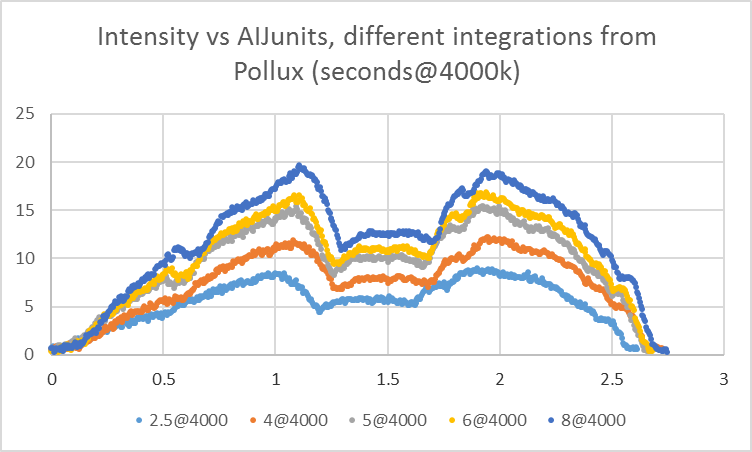
\includegraphics{saturation}
		\caption{Saturation plot, Pollux ($\beta$ Gem)}\label{fig:1}
	\end{figure}
	
	\subsection{White Balance}
	
	\begin{figure}[!h]
		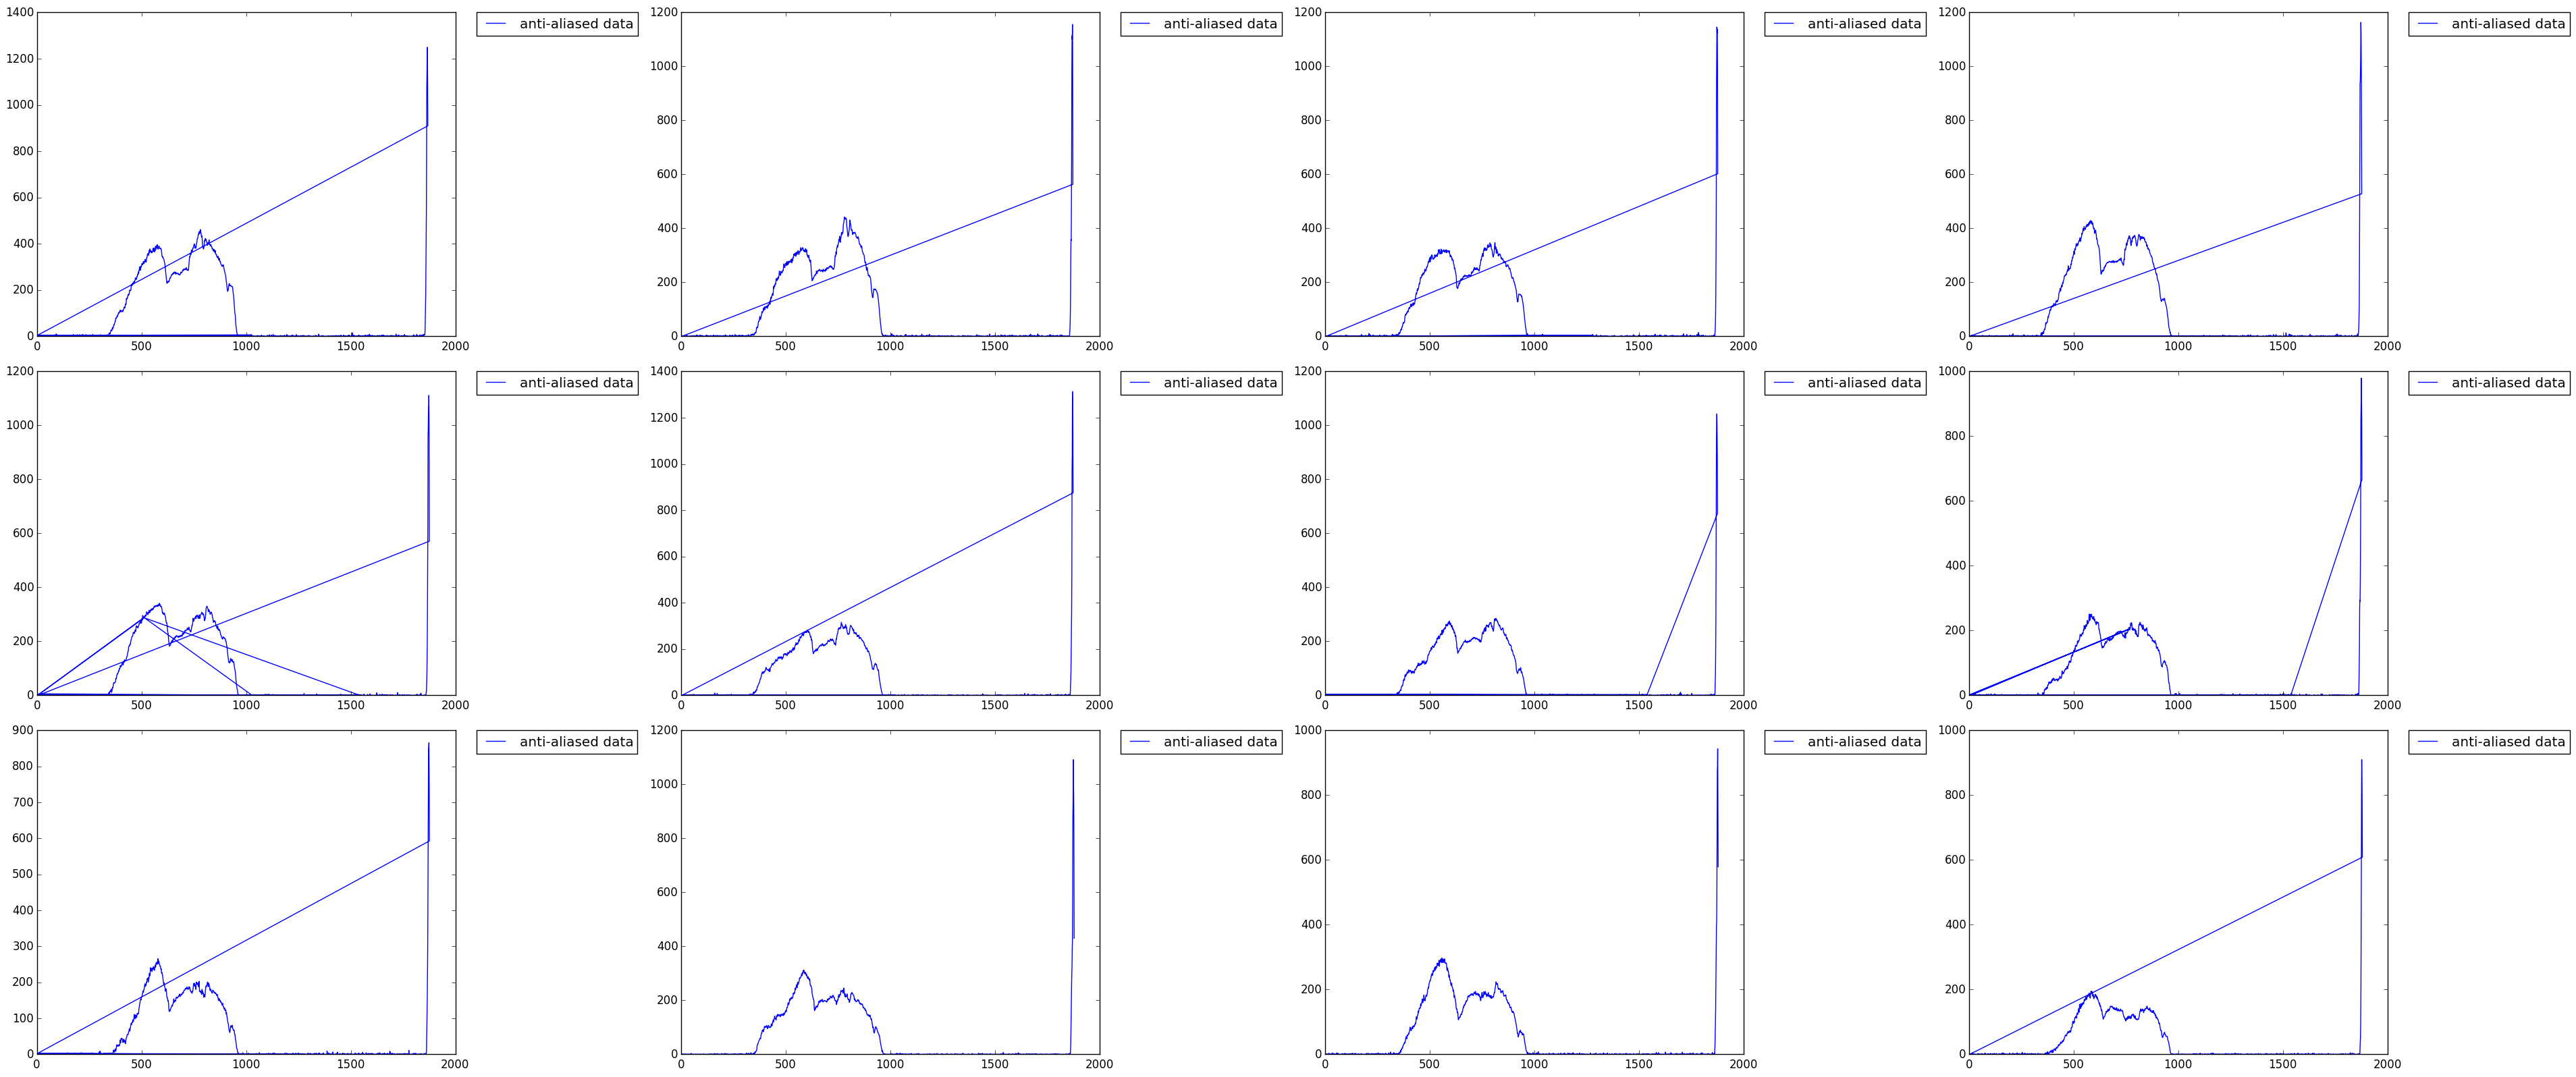
\includegraphics[keepaspectratio,scale=.132]{allLTR-UTD.jpg}
		\caption{White balance comparison. Row 1: 3000k, 3500k, 4000k, 4500k; Row 2: 5000k, 5500k, 6000k, 6500k; Row 3: 7000k, 7500k, 8000k, 8500k, Sirius A ($\alpha$ CMa A)}\label{fig:2}
	\end{figure}
	
	\subsection{Collection Procedure}
\section{Algorithms}
	Our final intensity plotting function, \verb|intensitySAAN| uses a form of spatial antialiasing (SAA) called super-sampling antialiasing. It is a very simple form of antialiasing where each pixel on a line is sampled at sub-pixel rates. Here, we calculate a line for each pixel along the x-axis of our image. Once we have that pixel, we then calculate the respective y-pixel using the m and c values obtained from the spectral regression. The resulting (x1,y1) pair is then a point along the spectral trace. We also calculate the line perpendicular to the spectral trace along the cross-dispersion axis by using $n = -1/m$ and a modified point-slope form equation $y = n \cdot (x \mathbb{-} x_1) + y1$. For sub-pixels (currently sampling at tenths of a pixel) located along this line, we calculate the percentage of the sub-pixel which lies along the line we have calculated. The full pseudocode algorithm can be referenced as algorithm \ref{alg:1} on page \pageref{alg:1}.
	
\section{Workflow Notes and Recommendations}
	stellarPYL contains an automated image processing workflow called \verb|autoProcess|, which is the simplest method of converting images from raw spectral data to intensity plots. In order to run this workflow, install Python 3.4, numpy, matplotlib, and Pillow (Python Imaging Library fork), or, alternately, simply install the Anaconda scientific computing Python distribution (making sure to use Python 3.4), which contains all the aforementioned libraries.
	
	Run \verb|python ui.py| making sure to place your image in the same folder as \verb|ui.py|. 
	
	We have implemented a multi-use threshold value which persists across sessions. This threshold determines what the program sees as pertinent or useful data. The value can range from 0--765, where anything above the value is considered pertinent. The default for this threshold is 127. In order to get a sense of the distribution of pixel values in your image, you can type \verb|pixel_d| and follow the prompts.
	
	In order to set the new default threshold, type \verb|settings_threshold| and the prompts will guide you through the process of setting a new threshold. After setting this threshold, we can begin the \verb|autoProcess|. The cropping function will automatically crop the image. If you find any parts of your image are being cropped off, you can set a manual row or column to stop the crop.

	blah blah
\section{Spectral Sensitivity Correction}
	bah
	\subsection{Absolute Response Function}
		bah
	\subsection{Relative Response Function}
		bah
\section{Conclusion}
	bah
	
\section{Acknowledgments}
	We acknowledge St. Paul's School for funding via the Thomas Penrose Bennett Prize of 2014. We also recognize Scott Silver and Evan Sinukoff for programming assistance. Finally, Brunston Poon thanks Dr. \@Mathews for his assistance throughout the entire process.

\section{Appendix A}

\begin{algorithm}[!h]
	\begin{algorithmic}
		\STATE \textbf{ARGUMENTS}: (image, imagedata, m, c, threshold, step)
		\STATE set medianbackground = backMedian(image)
		\STATE initialize intensity dictionary $i\{\}$
		\STATE set n = $-1 / m$\;
		\FOR{x \emph{in} image bounds at rate of 1 pixel}
		\STATE set y = $m \cdot x + c $
		\FOR{new\_x \emph{in} image bounds at rate of 0.1 pixel}
		\STATE set new\_y = $n \cdot (new\_x - x) + y $
		\IF{new\_y \emph{in} image bounds}
		\FOR{x\_rounded \emph{in} (floor(x),ceil(x))}
		\FOR{y\_rounded \emph{in} (floor(y),ceil(y))}
		\IF{y\_rounded \emph{in} image bounds}
		\STATE //determining percentage of pixel occupying region
		\STATE set percent\_x = $1 - abs(new\_x - x\_rounded$
		\STATE set percent\_y = $1 - abs(new\_y - y\_rounded)$
		\STATE set total\_percent = $percent\_x + percent\_y$
		\STATE get pixel at (x\_rounded, y\_rounded) from 	image
		\STATE set pixel\_value = $total\_percent \cdot pixel\_value$
		\IF{value already set at this pixel}
		\STATE set i[x] = $i[x] + pixel\_value$
		\ELSE
		\STATE set i[x] = $pixel\_value$
		\ENDIF
		\STATE set i[x] = $i[x] - percent \cdot median background$
		\ENDIF
		\ENDFOR
		\ENDFOR
		\ENDIF
		\ENDFOR
		\ENDFOR
		\STATE \textbf{RETURN:} intensity dictionary $i\{\}$
	\end{algorithmic}
	\caption{\emph{Intensity calculation function with spatial anti-aliasing.}}\label{alg:1}
\end{algorithm}

\begin{thebibliography}{99}
	
	\bibitem{5dspec} Canon manufacturer specifications for EOS 5D, \verb|<http://goo.gl/Rh2zVj>|.
	
	\bibitem{12232} ISO 12232, Determination of exposure index, ISO speed ratings, standard output sensitivity, and recommended exposure index, \verb|<http://goo.gl/JX8Wl8>|.
	
	\bibitem{paton} Paton Hawksley SA-100 information, \verb|<http://goo.gl/bwk92L>|.
	
	\bibitem{fc125spec} Takahashi data sheet (for FC-125 specifications), \verb|<http://goo.gl/1C07aP>|.
	
	\bibitem{vbpdslr} Kloppenborg, B. K.; Pieri, R.; Eggenstein, H.-B.; Maravelias, G.; Pearson, T., "A Demonstration of Accurate Wide-field V-band Photometry Using a Consumer-grade DSLR Camera," JAAVSO \textbf{40} (2), 815-833 (2012).
	
	\bibitem{mbpdslr} Zhang, M.; Bakos, G. Á.; Penev, K.; Csubry, Z.; Hartman, J. D.; Bhatti, W.; de Val-Borro, M., "Precision multi-band photometry with a DSLR camera," eprint arXiv:1506.03097, (2015).
	
\end{thebibliography}
\end{document}